\subsection{Case Study}
\label{sec:eval}

Now in this section, we study the overall cost for placing datacenters and renewable energy power plants into the same grid network. By considering the grid loss or not, we can get different results of placement decisions.

\thunote{Moved the following text here from previous section.  Need to integrate.}

datacenters and renewable power plant, as well as the capacity provisioned at each location for datacenters or green power plants (if any).

Equation 24 means that the provisioned capacity for renewable energy plants are determined by the total power demand from the datacenters. This constraint is added indicating that the power generation and consumption added to the grid should be balanced from the perspective of the grid system.

\thunote{End of moved text.}

\subsubsection{Input data}

The target area here is New England in United States, and we select 56 locations as candidates inside this area, as shown in Figure \ref{fig:NE_locs}. We obtained the Typical Meteorological Year (TMY) information for 56 locations from US Department of Energy (2), which includes a one-year dataset of hourly weather values for a location. We simplify the problem by only considering one type of renewable energy - wind. We computed the average wind power generation using $\beta(l,t)$ derived from the specifications for the 1.5MW Series wind turbine from General Electric Company \cite{GE15MW}, TMY wind speed, TMY air pressures, and conversion losses.

Besides, we collected various data of PUEs, datacenter construction costs, wind farm construction costs, land costs, transmission lines and network connection costs and grid energy costs in the same way as stated in \cite{berral2014building}. Specifically, for grid costs, we use $priceLoss$ the same as the maximum electricity price in the whole area. The input data for the grid is derived from the New England grid system, which is shown as in Section \ref{sec:quantify},including all of the settings for buses, branches and generators in it. Thus, the transmission loss, $transLoss(t)$, could be computed by simulating the power flow process for time epoch $t$.  %According to the study in \cite{aman2012ITPD}, we set the distribution loss as 3\% of the average power generation of the added power plant.


\begin{figure}[ht]
\centering
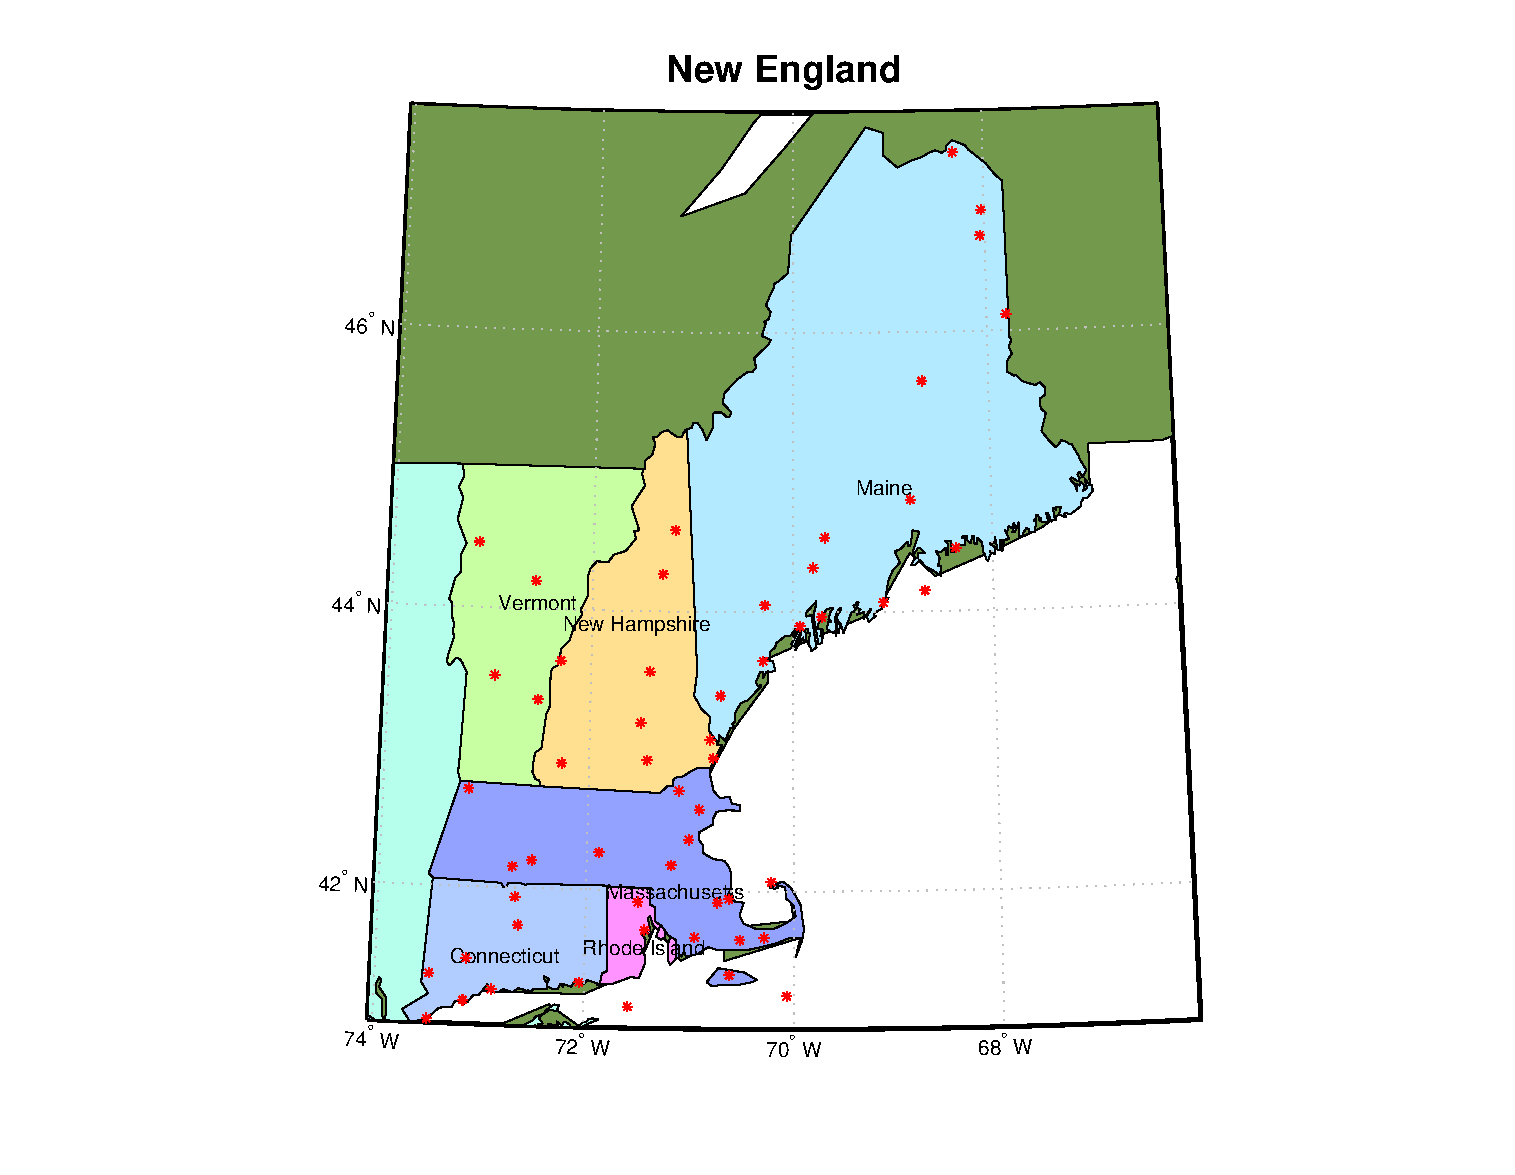
\includegraphics[width=1\columnwidth]{img/NE_map}
\caption{Candidate locations in New England}
\label{fig:NE_locs}
\end{figure}

\subsubsection{Building one datacenter with one wind farm}

Here, we are trying to solve a simplest case of the defined problem by placing only one datacenter and only one wind farm onto the grid system. The added generation (wind power) and consumption (datacenter load) should be balanced for the grid to keep reliability to the best extent. In this case, we can brute force all of the combinations of locations for the datacenter and the wind farm. Figure \ref{fig:cost1dc1wf} shows the results of the total cost by using five different strategies when seeking the best locations when we are building a 100MW datacenter and a wind farm which can supply green energy for it.

\begin{figure}[ht]
\centering
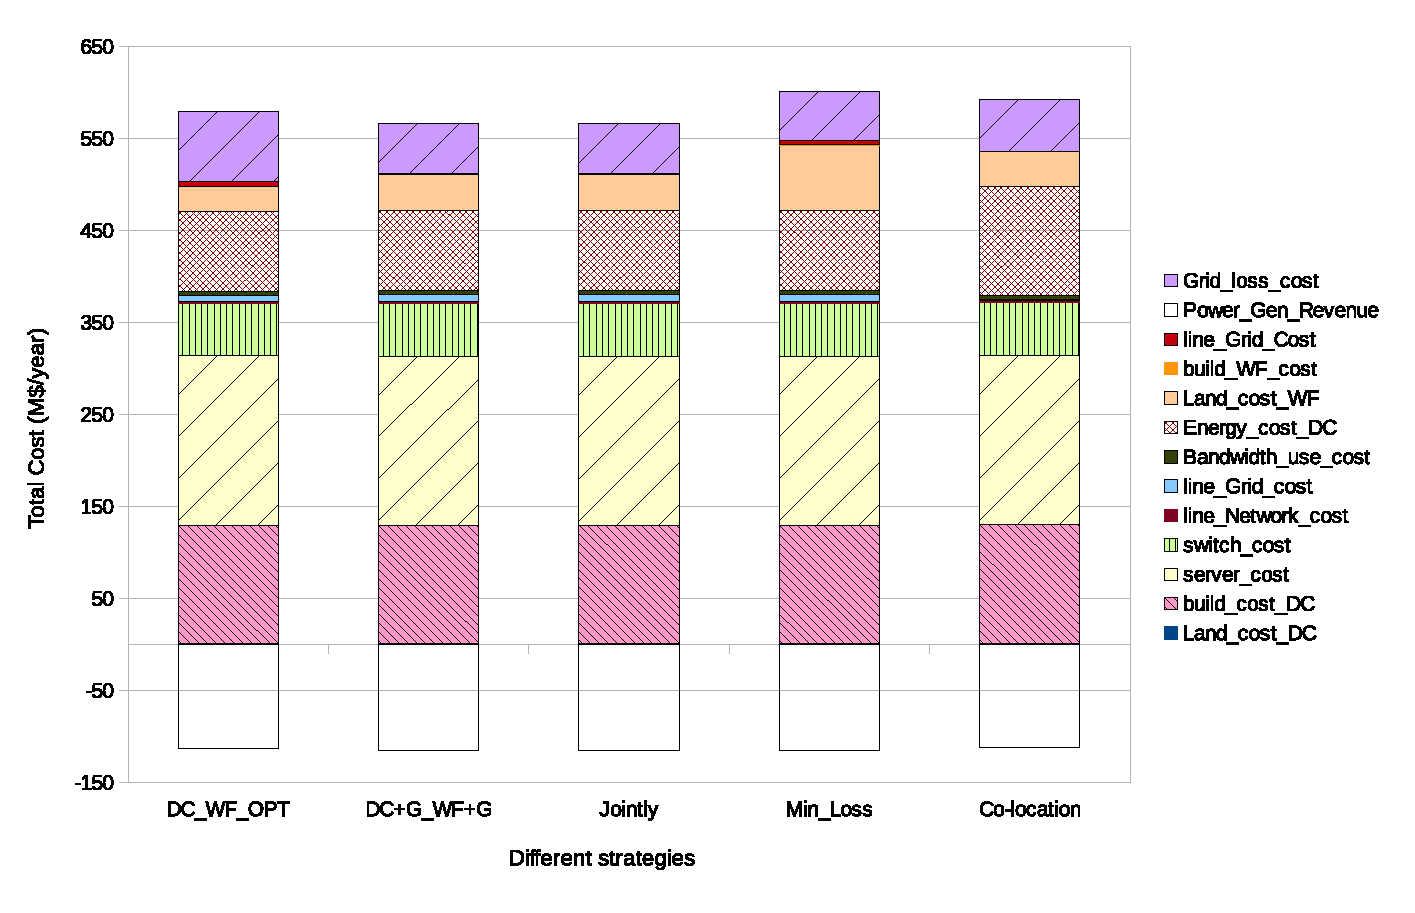
\includegraphics[width=1\columnwidth]{img/cost-one-dc-one-wf}
\caption{Costs of building one datacenter (100MW) with one wind farm}
\label{fig:cost1dc1wf}
\end{figure}

The five different strategies are explained as follows:

(1)\textbf{DC\_WF\_OPT.} This strategy tries to seek for the best location for the datacenter where its total cost could be minimized, and the best location for the wind farm where its total cost could be minimized. \xynote {According to Divya, today there are standard methods used to determine the best location for wind farms. So are you suggesting us to focus on the placement of datacenters only? } Grid costs are not considered here.

(2)\textbf{DC+G\_WF+G.} Since only putting datacenter or wind farm into the grid will change the power flow, this strategy tries to add the transmission loss costs into consideration when seeking for best locations separately for the datacenter and the wind farm.

(3)\textbf{Jointly.} All of the combinations of locations are exploited by using this strategy to seek for the jointly placement choice for both the datacenter and the wind farm, considering the total cost as calculated by Equation 2.

(4)\textbf{Min\_Loss.} Here, this strategy seeks for the locations for datacenter and wind farm which can lead to the minimal grid losses cost.

(5)\textbf{Co-location.} Assuming the the datacenter should be build together with an on-site wind farm, this strategy seeks for one location to place both the datacenter and the wind farm towards minimizing the total cost.

From the figure, we can see that by considering grid costs, the total cost will be further saved compared to best choices for the datacenter and the wind farm separately. Also, $Min\_Loss$ can achieve minimal losses of all possible choices, but the total cost is large mainly because it selects an expensive place for purchasing land for the wind farm. The best choice of co-location options is also nearly 7\% higher than the $Jointly$ choice, and it's easy to understand since the best location for datacenter is not necessarily the best for wind farm and vice versa.

We calculate all of the combinations for wind farm and datacenter locations and use the average total cost of these combinations (which is \$667.1M per year) as the baseline for comparison. Then, the locations found and the corresponding cost savings of the five strategies are listed in Table \ref{tab:costsaving}.

\begin{table}[ht]
\begin{center}
\caption{Detailed results of cost savings by different strategies.}
\begin{tabular}{|l|p{50pt}|p{50pt}|p{30pt}|p{20pt}|}
\hline
\textbf{Strategy}& \textbf{Datacenter location} &\textbf{Wind farm location} &\textbf{Total cost (M\$/year)} &\textbf{Cost saving (\%)} \\
\hline
\textbf{DC\_WF\_OPT} &  Burlington,NH  & Mount Washington, NH &465.6& 30.2 \\
\textbf{DC+G\_WF+G} &Springfield Hartnes, VT  & Nash Island, CO&450.3& 32.5\\
\textbf{Jointly} &Springfield Hartnes, VT&  Nash Island, CO & 450.3 & 32.5\\
\textbf{Min\_Loss} &Springfield Hartnes, VT & Marthas Vineyard, RI & 485.6& 27.2 \\
\textbf{Co-location}& Nash Island, CO &Nash Island, CO&480.7 & 27.9  \\
\hline
\end{tabular}
\label{tab:costsaving}
\end{center}
\end{table}
